\documentclass[aspectratio=169]{beamer}
\usepackage{tikz}
\usetikzlibrary{shapes.geometric}
\usetikzlibrary{arrows}
\usepackage{amsmath,amssymb}
\usepackage{array}
\usepackage{graphbox}
\usepackage{xcolor}

\newcommand{\yicon}{\includegraphics[width=20px]{icon-check.png}}
\newcommand{\nicon}{\includegraphics[width=20px]{icon-cross.png}}

\setbeamertemplate{footline}[frame number]
\setbeamertemplate{navigation symbols}{}

\setbeamercolor{palette primary}{fg=black,bg=white}
\setbeamercolor{palette secondary}{fg=black,bg=white}
\setbeamercolor{structure}{fg=black,bg=white}

% title frame
\defbeamertemplate*{title page}{mytheme}[1][]
{
  \begin{tikzpicture}[remember picture,overlay]
  \filldraw[white]
    (current page.north west) --
    (current page.north east) --
    ([xshift=0cm,yshift=-2cm]current page.north east)  --
    ([xshift=0cm,yshift=-2cm]current page.north west) -- cycle
    ;
  
  \node[opacity=0.1] at ([xshift=-2.5cm,yshift=-0.3cm]current page.north east) {\includegraphics[width=12cm]{wcc}};
  
  \node[text=black,anchor=south west,font=\sffamily\LARGE,text width=.8\paperwidth] at ([xshift=-100pt,yshift=-1cm]current page.center)(title){\raggedright\inserttitle};
    
  \node[text=black,anchor=south west,font=\sffamily\small,text width=.6\paperwidth] at ([xshift=-100pt,yshift=-1.5cm]current page.center)(institute){\raggedright\insertinstitute};
   
  \node[text=black,font=\large\sffamily,anchor=south west] at ([xshift=30pt,yshift=0.5cm]current page.south west)(date){\insertdate};
  
  \node[text=black,font=\large\sffamily,anchor=south west] at ([yshift=5pt]date.north west)(author){\insertauthor};
  \end{tikzpicture}
}

% definition of the symbols used in itemize
\newcommand\mysymbol{%
  \begin{tikzpicture}[xscale=0.85]
\draw[black, thick]  circle (1.5 pt);             
  \end{tikzpicture}%
  }

% definition of the itemize templates
\defbeamertemplate*{itemize item}{mysymbol}{\small\raise0.5pt\hbox{\mysymbol}}
\defbeamertemplate*{itemize subitem}{mysymbol}{\footnotesize\raise0.5pt\hbox{\mysymbol}}
\defbeamertemplate*{itemize subsubitem}{mysymbol}{\footnotesize\raise0.5pt\hbox{\mysymbol}}

\title[Transaction privacy: past, present, and future]{Transaction privacy: past, present, and future}
\author{Sarang Noether, Ph.D.}
\date{Halloween 2019}

\institute{World Crypto Con, Las Vegas}

\begin{document}

\begin{frame}[plain]
\maketitle
\end{frame}


\begin{frame}
\frametitle{Disclaimers}
\begin{columns}
\begin{column}{0.2\textwidth}
\includegraphics[width=0.9\textwidth]{icon-jack.png}
\end{column}
\begin{column}{0.8\textwidth}
The views expressed in this presentation are solely those of the author, and do not necessarily reflect those of any other person, organization, or community. \\~\\

The material in this presentation is for educational purposes only and should not be construed as financial, legal, or other professional advice, nor as endorsement of any kind. \\~\\

The author is an independent research mathematician who contributes to the Monero Research Lab workgroup and receives funding support from the Monero community.
\end{column}
\end{columns}
\end{frame}


\begin{frame}{Goals}
You should understand and appreciate:
\begin{itemize}
\item the \textbf{importance} of fungibility and privacy in transaction protocols
\item the \textbf{evolution} of cryptographic approaches used
\item \textbf{differences} between transaction models and proving systems
\item how \textbf{tradeoffs} in efficiency and trust affect design choices \\~\\
\end{itemize}

\begin{columns}
\begin{column}{0.2\textwidth}
\centering
\includegraphics[width=0.6\textwidth]{icon-ghost.png}
\end{column}
\begin{column}{0.6\textwidth}
\centering
The math gets spooky; you'll find none of it here.
\end{column}
\begin{column}{0.2\textwidth}
\centering
\includegraphics[width=0.6\textwidth]{icon-ghost.png}
\end{column}
\end{columns}
\end{frame}


\begin{frame}{Fungibility?}
Privacy and fungibility are related. \textbf{Fungibility} can mean indistinguishability. Can particular funds be blacklisted? \\~\\

Transparent ledgers like Bitcoin are highly non-fungible and non-private.
\begin{itemize}
\item Addresses appear on the chain as part of transactions
\item Amounts are in the clear
\item Assets have distinguishable history and properties
\end{itemize}

{\Huge $$\begin{array}{l} \includegraphics[width=40pt]{btc.png} \end{array} \quad \neq \quad  \begin{array}{l} \includegraphics[width=40pt]{btc.png} \end{array}$$}
\end{frame}


\begin{frame}{Transaction fundamentals}
Transactions (primarily) consist of \textbf{inputs}, \textbf{outputs}, and \textbf{authorizations}. \\~\\

A transaction consumes inputs using authorizations, and generates new outputs. A digital signature is the most basic authorization. \\~\\

\begin{figure}
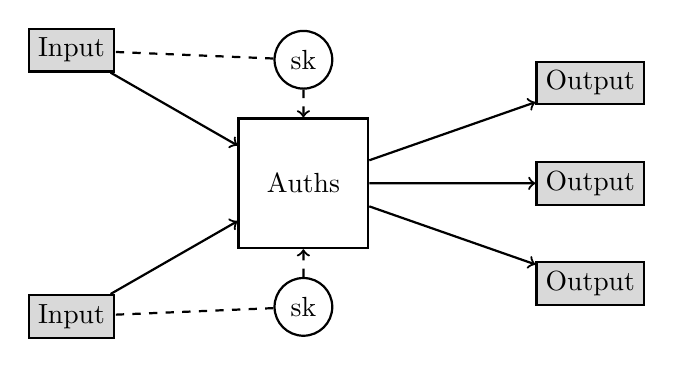
\begin{tikzpicture}[thick,square/.style={regular polygon,regular polygon sides=4}]
\node [square,draw] (auths) {Auths};
\node [rectangle,draw,left=60pt,above=40pt,at=(auths.west),fill=gray!30] (input1) {Input};
\node [rectangle,draw,left=60pt,below=40pt,at=(auths.west),fill=gray!30] (input2) {Input};
\node [circle,draw,above=10pt,at=(auths.north)] (sk1) {sk};
\node [circle,draw,below=10pt,at=(auths.south)] (sk2) {sk};
\node [rectangle,draw,right=60pt,at=(auths.east),fill=gray!30] (output2) {Output};
\node [rectangle,draw,above=20pt,at=(output2.north),fill=gray!30] (output1) {Output};
\node [rectangle,draw,below=20pt,at=(output2.south),fill=gray!30] (output3) {Output};

\draw [->] (input1) -- (auths);
\draw [->] (input2) -- (auths);
\draw [dashed,-] (sk1) -- (input1);
\draw [dashed,-] (sk2) -- (input2);
\draw [dashed,->] (sk1) -- (auths);
\draw [dashed,->] (sk2) -- (auths);
\draw [->] (auths) -- (output1);
\draw [->] (auths) -- (output2);
\draw [->] (auths) -- (output3);
\end{tikzpicture}
\end{figure}

\end{frame}


\begin{frame}{Transaction graph}
Any network participant can analyze a transparent ledger and examine the flow of funds through transactions. \\~\\

\begin{figure}
\includegraphics[width=0.7\textwidth]{btc-chain.png}
\end{figure}

A \underline{lot} of research has focused on methods of chain analysis using transparency.
\end{frame}


\begin{frame}{Why care?}
Transparency and non-fungibility have consequences that you may or may not like:

\begin{itemize}
\item \textbf{Censorship}: miners and other entities can censor transactions based on addresses, amount, location, or other transaction data/metadata
\item \textbf{Markets}: certain types or quantities of assets may fetch a market premium based on history or usage
\item \textbf{Linking}: any third party with access to the public chain can link data and amounts and attempt to link to identity, increasing personal risk
\item \textbf{Competition}: business competitors can trivially gain information about transactions that yields proprietary information or business data
\item \textbf{Regulations}: certain jurisdictions may impose rules requiring financial information be kept private in storage and transit \\~\\
\end{itemize}

The term ``privacy coin" has it reversed! Shouldn't all bathrooms have doors?
\end{frame}


\begin{frame}{Spectrum of common approaches}
\begin{figure}
\centering
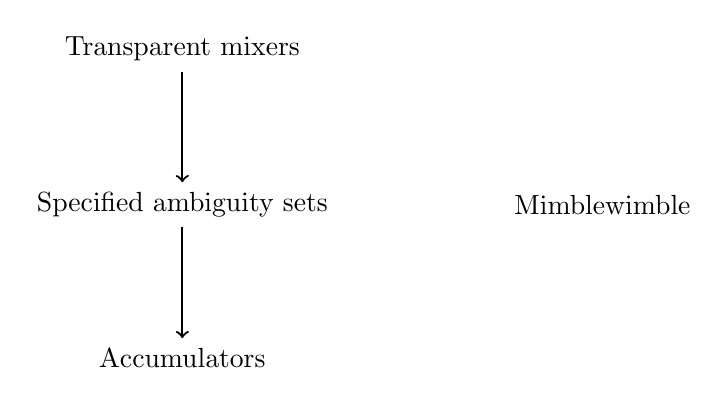
\begin{tikzpicture}[thick]
\node (mixers) {Transparent mixers};
\node [below=40pt,at=(mixers.south)] (decoys) {Specified ambiguity sets};
\node [below=40pt,at=(decoys.south)] (acc) {Accumulators};
\node [right=60pt,at=(decoys.east)] (mw) {Mimblewimble};

\draw [->] (mixers) -- (decoys);
\draw [->] (decoys) -- (acc);
\end{tikzpicture}
\end{figure}
\end{frame}


\begin{frame}{Example: transparent mixers}
\textbf{Transparent mixers} take transparent funds with possibly different owners and include them in the same transaction. Authorizations can be modified accordingly, but typically no new math.

\begin{figure}
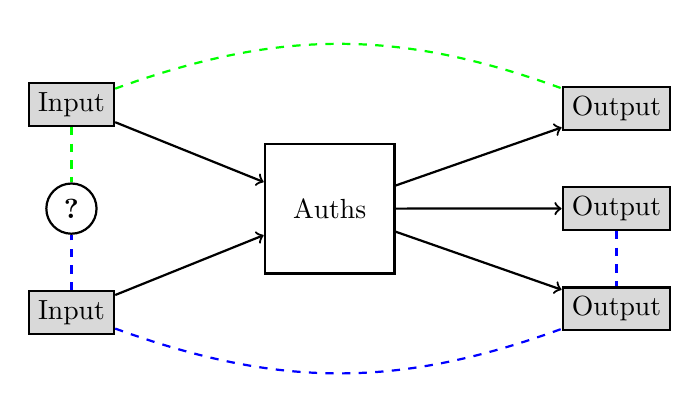
\begin{tikzpicture}[thick,square/.style={regular polygon,regular polygon sides=4}]
\node [square,draw] (auths) {Auths};
\node [circle,draw,left=60pt,at=(auths.west)] (q) {\textbf{?}};
\node [rectangle,draw,above=20pt,at=(q.north),fill=gray!30] (input1) {Input};
\node [rectangle,draw,below=20pt,at=(q.south),fill=gray!30] (input2) {Input};
\node [rectangle,draw,right=60pt,at=(auths.east),fill=gray!30] (output2) {Output};
\node [rectangle,draw,above=20pt,at=(output2.north),fill=gray!30] (output1) {Output};
\node [rectangle,draw,below=20pt,at=(output2.south),fill=gray!30] (output3) {Output};

\draw [->] (input1) -- (auths);
\draw [->] (input2) -- (auths);
\draw [->] (auths) -- (output1);
\draw [->] (auths) -- (output2);
\draw [->] (auths) -- (output3);
\draw [dashed,-,green] (input1) -- (q);
\draw [dashed,-,blue] (input2) -- (q);
\draw [dashed,-,green] (input1) to [out=20,in=160] (output1);
\draw [dashed,-,blue] (input2) to [out=-20,in=-160] (output3);
\draw [dashed,-,blue] (output2) -- (output3);
\end{tikzpicture}
\end{figure}

\end{frame}


\begin{frame}{Example: transparent mixers}
\begin{columns}
\begin{column}{0.7\textwidth}
Upsides:
\begin{itemize}
\item Breaks assumption of common ownership \\~\\
\end{itemize}

Downsides:
\begin{itemize}
\item Little-to-no privacy for senders or recipients
\item Interactive, opt-in process
\item Does not provide fungible assets, only uncertainty
\item Many analysis methods still apply as usual
\end{itemize}
\end{column}
\begin{column}{0.3\textwidth}
\begin{figure}
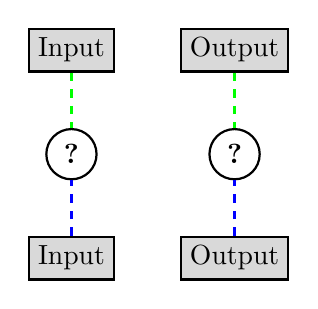
\begin{tikzpicture}[thick]
\node [circle,draw] (q) {\textbf{?}};
\node [rectangle,draw,above=20pt,at=(q.north),fill=gray!30] (input1) {Input};
\node [rectangle,draw,below=20pt,at=(q.south),fill=gray!30] (input2) {Input};


\node [circle,draw,right=40pt,at=(q.east)] (q2) {\textbf{?}};
\node [rectangle,draw,above=20pt,at=(q2.north),fill=gray!30] (output1) {Output};
\node [rectangle,draw,below=20pt,at=(q2.south),fill=gray!30] (output2) {Output};

\draw [dashed,-,green] (input1) -- (q);
\draw [dashed,-,blue] (input2) -- (q);
\draw [dashed,-,green] (output1) -- (q2);
\draw [dashed,-,blue] (output2) -- (q2);
\end{tikzpicture}
\end{figure}
\end{column}
\end{columns}
\end{frame}


\begin{frame}{Example: RingCT}
\textbf{RingCT} is a protocol that uses a set of constructions, implemented in Monero and elsewhere. It uses one-time addresses to mitigate (but not eliminate) linking. Ambiguous signatures sign on behalf of a sender-chosen group of possible spends. Amounts are hidden using Pedersen commitments. \\~\\

\begin{columns}
\begin{column}{0.2\textwidth}
\includegraphics[width=\textwidth]{ambiguous.png}
\end{column}
\begin{column}{0.8\textwidth}
Taken together, these provide limited sender ambiguity, recipient anonymity, and amount hiding toward fungibility.
\end{column}
\end{columns}
\end{frame}

\begin{frame}{Example: RingCT}
\begin{columns}
\begin{column}{0.7\textwidth}
Upsides:
\begin{itemize}
\item Replaces undeniable signatures with ambiguous signatures
\item Hides amounts
\item Obscures transaction graph \\~\\
\end{itemize}

Downsides:
\begin{itemize}
\item Metadata can reduce effective anonymity
\item Scaling is inefficient
\item Does not fully remove common-ownership heuristic
\end{itemize}
\end{column}
\begin{column}{0.3\textwidth}
\begin{figure}
\includegraphics[width=0.8\textwidth]{ambiguous.png}
\end{figure}
\end{column}
\end{columns}
\end{frame}


\begin{frame}{Example: Zerocoin}
\textbf{Zerocoin} is/was the first serious accumulator approach to fungibility as an extension to transparent ledgers. It was used in assets like Zcoin (not anymore!) but is considered broken. \\~\\

\begin{figure}
\includegraphics[width=0.7\textwidth]{zerocoin-chain.png}
\end{figure}

You \textbf{mint} a Zerocoin by burning known Bitcoin and adding to a coin accumulator. You \textbf{spend} a Zerocoin by proving ownership of an unknown accumulator coin, transferring to Bitcoin.
\end{frame}


\begin{frame}{Example: Zerocoin}
\begin{columns}
\begin{column}{0.7\textwidth}
Upsides:
\begin{itemize}
\item Accumulator ensured maximal spend ambiguity
\item Could play nicely with transparent assets \\~\\
\end{itemize}

Downsides:
\begin{itemize}
\item Possible to burn honest users' funds upstream
\item Flawed mint proof exploited for inflation
\item Limited to fixed amounts with no direct transfer
\item Large and inefficient proofs
\item Timing and linking carry over to main chain
\end{itemize}
\end{column}
\begin{column}{0.3\textwidth}
\begin{figure}
\includegraphics[width=0.6\textwidth]{zerocoin.png}
\end{figure}
\end{column}
\end{columns}
\end{frame}


\begin{frame}{Zerocash/Zcash}
\textbf{Zerocash} was a transaction protocol that influenced the \textbf{Zcash} protocols. Current protocols use Merkle tree accumulators, but with much greater flexibility than Zerocoin due to more robust proof systems. \\~\\

Transactions support direct transfers of hidden amounts, hiding spends within the accumulator. Privacy is optional.

\begin{figure}
\includegraphics[width=0.4\textwidth]{zcash-types.png}
\end{figure}
\end{frame}


\begin{frame}{Example: Zerocash/Zcash}
\begin{columns}
\begin{column}{0.7\textwidth}
Upsides:
\begin{itemize}
\item Accumulator ensures maximal spend ambiguity
\item Can play nicely with transparent assets
\item Supports direct transfers
\item Small proofs with verification efficiency \\~\\
\end{itemize}

Downsides:
\begin{itemize}
\item Proving system soundness requires non-collusion and correct MPC
\item Complex structure due to more general proving systems
\item Optional privacy
\item Transitions admit linking and timing analysis
\end{itemize}
\end{column}
\begin{column}{0.3\textwidth}
\begin{figure}
\includegraphics[width=0.6\textwidth]{zcash.png}
\end{figure}
\end{column}
\end{columns}
\end{frame}


\begin{frame}{Why so many approaches?}
\begin{itemize}
\item \textbf{Transparent mixing} offers effectively \textit{no} privacy and very limited fungibility, but retains general compatibility with transparent ledgers using interactive processes.
\item \textbf{Obfuscation/ambiguity} designs can provide reasonable sound privacy and fungibility, but at the cost of efficiency and some graph analysis.
\item \textbf{General proving systems} can be used to built small and fast transactions for accumulator-based transaction models with good privacy, but practically at the cost of soundness guarantees. \\~\\
\end{itemize}
\end{frame}


\begin{frame}{Transaction model vs. proving system}
A \textbf{transaction model} is a collection of cryptographic constructions (signatures, proofs) used to demonstrate things like asset ownership, non-double-spending, balance, destination, and so on. We've seen several. \\~\\

A \textbf{proving system} is a cryptographic construction used to prove and verify mathematically-defined statements involving private and public data, ideally in zero knowledge. Some work on specific statements, and others are more general. \\~\\

\begin{itemize}
\item Having a proving system does not give you a transaction model. A language is useless if you have nothing to say.
\item The constructions in some transaction models can be built using proving systems to produce and verify transactions, but this has many caveats relating to efficiency and specificity. The nature of the reference string plays a large role (e.g. for Zcash and related assets).
\end{itemize}
\end{frame}


\begin{frame}
\begin{figure}
\includegraphics[width=\textwidth]{puzzle.jpeg}
\end{figure}
\end{frame}


\begin{frame}{Metadata matters}
\begin{table}
\centering
\begin{tabular}{>{\arraybackslash}m{0.3in} >{\arraybackslash}m{2.0in}}
\includegraphics[width=20px]{icon-earth.png} & Network/location data \\
\includegraphics[width=20px]{icon-web.png} & Transaction relay \\
\includegraphics[width=20px]{icon-arrows.png} & Input/output structure \\
\includegraphics[width=20px]{icon-stopwatch.png} & Timing/periodicity \\
\includegraphics[width=20px]{icon-clip.png} & Address linking \\
\includegraphics[width=20px]{icon-bike.png} & Migrations/transitions \\
\includegraphics[width=20px]{icon-spy.png} & Side-channel attacks
\end{tabular}
\end{table}

\begin{center}
\textbf{The best transaction models in the world do not remove all metadata!}
\end{center}
\end{frame}


\begin{frame}{Research directions}
\begin{figure}
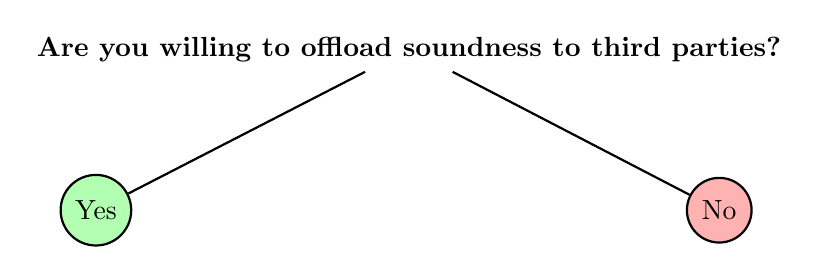
\begin{tikzpicture}[thick]
\node (q) {\textbf{Are you willing to offload soundness to third parties?}};
\node [circle,draw,below=50pt,left=100pt,at=(q.south),fill=green!30] (yes) {Yes};
\node [circle,draw,below=50pt,right=100pt,at=(q.south),fill=red!30] (no) {No};

\draw [-] (q) -- (yes);
\draw [-] (q) -- (no);
\end{tikzpicture}
\end{figure}
\begin{columns}
\begin{column}{0.5\textwidth}
There are good proving systems on which you can build fast and efficient transaction protocols for accumulator-based anonymity and privacy.
\end{column}
\begin{column}{0.5\textwidth}
The options are mostly ad-hoc and suffer from scaling problems for signature and proof sizes. Verification typically scales as least as badly as size.
\end{column}
\end{columns}
\end{frame}


\begin{frame}{Example: MMORPG (Zcash Sapling)}
\textbf{MMORPG} is a variation by Bowe \textit{et al.} of a proving system by Groth. It proves statements about circuit satisfiability in zero knowledge. \\~\\

A structured/trusted setup is required, but is distributed. Proof size is less than 200 bytes for any circuit complexity. Proving is linear in the circuit complexity, but verification is linear only in the witness complexity. \\~\\

For the Zcash Sapling circuit, proving time is $O(1)$ seconds, and verification time is $O(1)$ milliseconds. (Proving time here relies on non-general circuit optimizations!) \\~\\

Used in:
\begin{figure}
\includegraphics[height=50pt]{zcash.png}
\end{figure}
\end{frame}


\begin{frame}{Example: Bulletproofs}
\textbf{Bulletproofs} are an extention by B\"{u}nz \textit{et al.} of an underlying proving system by Bootle \textit{et al.} to prove statements about circuit satisfiability in zero knowledge. \\~\\

There is no structured or trusted setup; reference strings are generated publicly. Size is logarithmic (sublinear) in the circuit complexity, but proving and verification are linear. \\~\\

For \underline{estimates} of the Zcash Sapling circuit, proving time is $O(10)$ seconds and verification time is $O(1)$ seconds (down to $O(100)$ milliseconds) for a proof of size $O(1)$ kB. \\~\\

Used in (optimized range proving only):
\begin{figure}
\includegraphics[align=c,height=42pt]{logo-beam.png}
\includegraphics[align=c,height=55pt]{logo-grin.png}
\includegraphics[align=c,height=50pt]{logo-monero.png}
\end{figure}
\end{frame}


\begin{frame}{Wild oversimplification}
\begin{table}
\centering
\begin{tabular}{>{\arraybackslash}m{1.0in} >{\arraybackslash}m{0.5in} >{\arraybackslash}m{0.5in} >{\arraybackslash}m{1.0in}}
& Bowe\footnote{IACR 2017/1050} & B\"{u}nz\footnote{IACR 2017/1066} & Ben-Sasson\footnote{IACR 2018/046} \\
\hline
Trust-free & \nicon & \yicon & \yicon \\
Small proof & \yicon & \yicon & \nicon \\
Fast proving* & \nicon & \nicon & \nicon \\
Fast verifying & \yicon & \nicon & \yicon
\end{tabular}
\end{table}
\begin{center}
* highly dependent on implementation and circuit
\end{center}
\end{frame}


\begin{frame}{The goal}
State-of-the-art research seeks to produce \textbf{general proving systems} with \textbf{no trust requirements} for soundness and \textbf{practical efficiency}. \\~\\

Some interesting work uses a universal and/or updateable reference string, but this has subtle implications for the trust model. \\~\\

\begin{center}
\textbf{It's trickier than it sounds, even if it already sounds tricky.}
\end{center}
\end{frame}


\begin{frame}{Thank you}
\textbf{Questions are welcome.} \\~\\

Transaction privacy and asset fungibility are tricky and unsolved, so please ask away. \\~\\

\begin{center}
\Large \texttt{sarang.noether@protonmail.com}
\end{center}
\end{frame}

\end{document}